\chapter{Square cylinder}
The square cylinder problem studies the two-dimensional laminar flow around a square cylinder inside a plane channel. The description of the problem can be seen in figure \ref{SchemeSquareProblem}.
\begin{figure}[h]
	\centering
	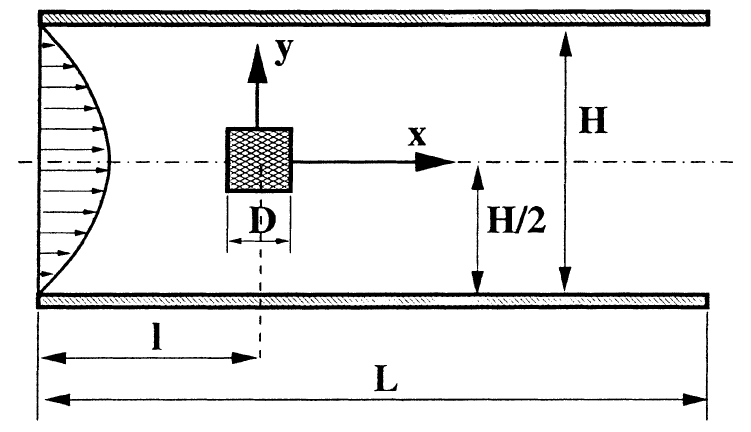
\includegraphics[scale=0.5]{Square/Definition}
	\caption[General scheme of the square cylinder problem]{General scheme of the square cylinder problem. Extracted from \cite{Breuer2000}}
	\label{SchemeSquareProblem}
\end{figure}

\section{Discretization}
In this kind of problem, the region near the cylinder has an important pressure and velocity gradient whereas in the rest of the channel flow they are smoother. So, near the cylinder a finer mesh is needed, but not in the whole domain of the problem. Using a very fine mesh in all the channel would be computationally expensive and inefficient, but a coarser mesh would lead to inaccurate results, especially in the cylinder.


\section{Boundary conditions}
\subsection{Inlet conditions}
Since the flow is inside a channel, the inflow has a parabolic velocity profile with a maximum velocity $u_{max}$ in the centre:
\begin{equation}
u\left(y\right)=4u_{max}\left[\left(\frac{y}{H}\right)-\left(\frac{y}{H}\right)^{2}\right]
\end{equation}
This maximum velocity defines the Reynolds number of the problem:
\begin{equation}
Re=Re_{max}=\frac{\rho u_{max}D}{\mu}
\end{equation}

\subsection{Outlet conditions}
In order to have a developed flow in the outlet, it is important to have a distance large enough between the position of the cylinder and the end of the channel in order to have fully developed flow. To define the outflow, a convective boundary condition is used:
\begin{equation}
\frac{\partial u}{\partial t}+u_{conv}\frac{\partial u}{\partial x}=0
\end{equation}
where $u_{conv}$ is equal to the maximum velocity $u_{max}$ of the parabolic inflow velocity profile.

\subsection{Wall conditions}
In the channel walls the no-slip condition is applied:
\begin{equation}
\vec{v}=0
\label{noslip}
\end{equation}
Another important condition is the boundary layer condition, in which the pressure gradient normal to the wall is 0.

In the convection problems studied in the previous sections the flow was developing inside a cavity with no other obstacles than the walls. In this problem, the fluid flows around a square cylinder, so some boundary conditions have to be also implemented for the cylinder. Since it is a solid object and it does not allow air to flow through it, it is treated as a wall \cite{Ferziger2002}. So the velocity in its boundary is given by equation \ref{noslip}.

This condition can also be interpreted using flow fluxes. To define the cylinder, it is determined that there are no flow fluxes through it. In the control volumes of the left wall, $F_{e}=0$, in the CVs of the right wall $F_{w}=0$, in the top wall $F_{n}=0$, and at the bottom $F_{s}=0$.
\begin{figure}[h]
	\centering
	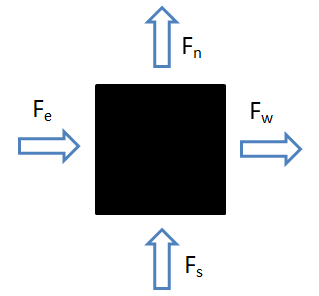
\includegraphics[scale=0.6]{Square/Fluxes}
	\caption{Fluxes conditions in the cylinder}
	\label{FluxesCondCylinder}
\end{figure}